\section{Esercizio 4}
\textit{\textbf{Descrizione:} Eseguire le seguenti istruzioni Matlab e spiegare i risultati ottenuti:\newline\newline		
format long e\newline
a = 1.111111111111111\newline
b = 1.11111111111111\newline
a + b\newline
a - b}\newline
\newline
\emph{Soluzione: }\\~\\

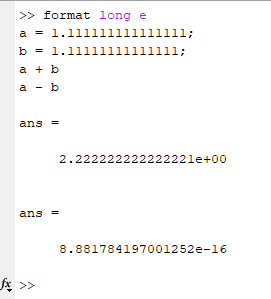
\includegraphics[width=.65\linewidth]{img/ex4}\\~\\
In questo script matlab vengono sommati due numeri $a$ e $b$ e poi viene fatta la differenza tra i due numeri $a$ e $b$.\\~\\
Nel caso della somma tra i due numeri il risultato ottenuto in Matlab corrisponde con il risultato ottenuto in matematica esatta in quanto una somma di numeri concorde \'e sempre ben condizionata poich\'e abbiamo
\begin{equation}
	\left | \varepsilon_{y}  \right | \leq \frac{\left | a \right | + \left | b \right |}{\left | a + b \right |} \varepsilon_{x} \equiv k \cdot \varepsilon_{x}
\end{equation}
in cui k \'e il numero di condizionamento
\begin{equation}
k =  \frac{\left | a \right | + \left | b \right |}{\left | a + b \right |}
\end{equation}
e per una somma di numeri concorde k=1 e quindi \'e sempre ben condizionata.
\\~\\
Nel caso della differenza tra i due numeri $a$ e $b$ invece il risultato ottenuto in Matlab differisce dal risultato ottenuto in matematica esatta perch\'e il risultato ottenuto, in matematica esatta, \'e \text{0.000000000000001} . In questo caso si verifica quindi il fenomeno della cancellazione numerica in cui si ha una perdita di cifre significative nel momento in cui viene effettuata una somma tra due numeri prossimi in valore assoluto ma opposti in segno. Infatti in questo caso, in cui $a \approx -b$, si ottiene un numero di condizionamento arbitrariamente grande e quindi l'operazione di somma algebrica risulta mal condizionata.
